\documentclass[../report]{subfiles}
\setcounter{section}{0}
\begin{document}

本章では,本プロジェクトの背景と目的を説明する.

\section{認知症の現状} \label{sec:genzyou}
近年の我が国では,認知症患者数が増加傾向にある.
二宮(2014)によると,2012年時点で日本国内の推定認知症患者数は462万人であった\cite{syourai}。2025年では675万人,2040年には802万人にまで上ると予想されている(図\ref{fig:nintisyo-graph}).
また同研究によると,65歳以上の高齢者の推定認知症有病率は2012年では15.5%,2025年には20.6%,2040年には25.4%と,年々増加傾向になさると予想されている\cite{syourai}.
また,認知症の発症には食生活や運動,睡眠といった生活習慣が関わっていることが明らかになっている\cite{seikatsu}.
\begin{figure}[htbp]
    \begin{center}
        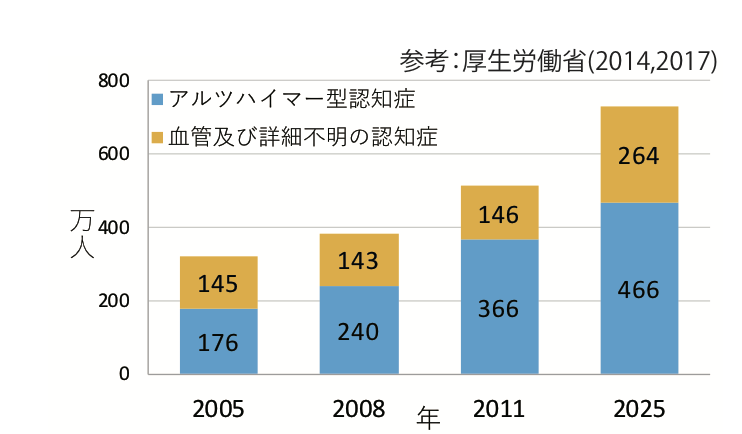
\includegraphics[width=10cm]{imgs/ninchisyo-graph.png}
        \caption{日本の認知症の総患者数の推移}
        \label{fig:ninchisyo-graph}
    \end{center}
\end{figure}
\bunseki{佐藤碧}

\section{現状における問題点} \label{sec:mondai}
 我が国では高齢化が進んでおり、今後もさらに進んでいくと予想されている中で,介護者不足が問題となっており,もはや高齢者は単なる庇護対象でいるだけでは不十分である\cite{kaigo}.むしろ積極的に自身の健康管理に関わっていき,病気の予防に努めるべきである.認知症予防のためには、\ref{sec:genzyou}でも上げたように自身の生活習慣を知り,問題があれば自身が改善することが重要になってくる.

 そのための手段としては、ライフログの記録・可視化といったことが挙げられ\cite{lifelog}、 一般にはICTが用いられている.ICTを利用する利点としては,蓄積した情報を管理・解析するのが容易であるということが挙げられる.しかし,高齢者の方はICTに苦手意識があったり,そもそも利用したことがないという方が多い.このように,高齢者の方にICTを利用したライフログ取得・管理をさせるには、利用しにくいといった問題がある.

 また,医療従事者が認知症の人の医療選択をする際に、判断材料が不足しているといった問題もある.従来の医療従事者が知り得た患者に関する情報は,診察から得られるその時点での情報に限定されていた.むしろ治療には,どのような過程で現状に至ったのかといったような長期的な情報が必要である.しかし現状では、それらを実現するような仕組みは未だ整備されていない.
\bunseki{佐藤碧}

\section{目的}
本グループでは、\ref{sec:mondai}で挙げた問題点を解決するために「ライフログの可視化による生活習慣の改善」、「ICTに不慣れな方でも容易にライフログを取得できる手段の開発」、「医療選択時に必要となる情報の蓄積」といったことを目指す。
\bunseki{佐藤碧}

\end{document}
